\documentclass[12pt,a4]{article}
\usepackage[left=1.8cm,right=1.8cm,top=32mm,columnsep=20pt]{geometry}

\usepackage[utf8]{inputenc} %Formato de codificación
\usepackage[spanish, es-tabla, es-nodecimaldot]{babel}
\usepackage{amsmath} %paquete para escribir ecuaciones matemáticas
\usepackage{float} %Para posicionar figuras
\usepackage{graphicx} %Para poder poner figuras
\usepackage{tikz}
\usetikzlibrary{positioning}
\usetikzlibrary{shapes.geometric, decorations.pathreplacing}

\title{Informe de Física: Encontrando el coeficiente de fricción dinámica}
\author{Francisco Carruthers, Facundo Firpo y Joel Jablonski\\ [2mm]
\small \texttt{\{fcarruthers, ffirpo, jjablonski\}@udesa.edu.ar}\\
\small Fisica I, tutorial Vinograd}
\date{2do Semestre 2024}


\begin{document}

\maketitle

\begin{abstract}
    Se investigó el coeficiente de fricción dinámica entre un carrito y varias superficies utilizando un sistema de carrito, soga y polea. Para garantizar la precisión de las mediciones, se realizó una calibración previa del sistema, ajustando los sensores y asegurando que las lecturas de posición y tiempo fueran precisas. A continuación, se varió la masa del carrito y se midió la aceleración para calcular el coeficiente de fricción dinámica ($\mu_d$) en diferentes superficies. Las superficies evaluadas incluyeron el carrito sobre madera, carrito sobre papel y papel sobre papel. Los valores obtenidos para el $\mu_d$ fueron: 0.4 ± 0.1 para madera y trineo, 0.45 ± 0.03 para papel y trineo, y 0.5 ± 0.2 para papel y papel. Los resultados demostraron que la superficie tiene un impacto significativo en la fricción dinámica del sistema.
\end{abstract}

\section{Introducción}

La fricción es una fuerza de resistencia que actúa en oposición al movimiento relativo entre dos superficies en contacto. Existen dos tipos principales de fricción: la fricción estática, que previene el inicio del movimiento, y la fricción dinámica (o cinética), que actúa cuando el objeto ya está en movimiento. En este experimento, nos centraremos en la fricción dinámica, cuyo coeficiente, denotado como \(\mu_d\), se define como la relación entre la fuerza de fricción y la fuerza normal ejercida sobre el objeto:

\[
F_r = \mu_d \cdot F_n
\]

donde \(F_r\) es la fuerza de fricción y \(F_n\) es la fuerza normal, que para superficies horizontales es equivalente al peso del objeto en contacto con la superficie. Este coeficiente depende del tipo de materiales en contacto y su textura.

La determinación del $\mu_d$ es fundamental en la física aplicada, ya que afecta el diseño de sistemas mecánicos, el análisis de movimientos y la estabilidad de objetos en distintas superficies. En este contexto, comprender la relación entre la fuerza de fricción y la aceleración del objeto es crucial. Para este experimento, utilizamos la segunda ley de Newton, que establece que la fuerza neta que actúa sobre un objeto es proporcional a la masa del objeto y su aceleración:

\[
F = m \cdot a
\]

Combinando esta ecuación con la expresión de la fuerza de fricción podemos deducir que la aceleración del carrito estará influenciada por el coeficiente de fricción y la masa total del sistema. Podemos despejar la formula como:

\begin{equation}
    \mu_d = \frac{a \cdot (M + m) + m \cdot g }{M \cdot g}
    \label{eq:mu_d}
\end{equation}

En nuestro caso, el sistema se conforma de un carrito y varias superficies, lo que nos permite explorar cómo el coeficiente de fricción cambia según el material.

El objetivo principal de esta práctica es medir el $\mu_d$ en diferentes superficies mediante el uso de un carrito y un sistema de polea. Para ello, se realizan mediciones de la aceleración y se compara cómo varía el coeficiente de fricción con el tipo de superficie y la masa utilizada. Este análisis teórico es esencial para comprender los resultados que se presentan en la sección siguiente.

Armamos el sistema de la siguiente manera:

\begin{figure}[H]
    \centering
    \begin{tikzpicture}
        % Dibuja la base
        \draw[thick] (-3,0) -- (1.5,0); % Línea base

        % Dibuja el trineo
        \node at (-0.8,0.78) {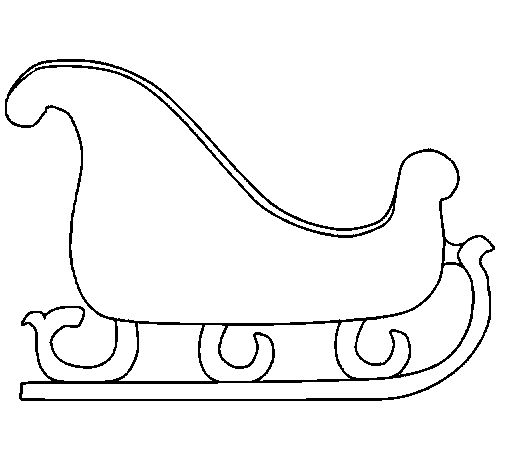
\includegraphics[height=1.5cm]{trineo.png} $M$} ; % Puedes añadir un símbolo del trineo aquí si tienes un archivo o usar símbolos de personajes ASCII.

        % Dibuja la cuerda que conecta al motor
        \draw[dashed] (-0.2,0.7) -- (2,0.7) -- (2,-2);
        
        % Dibuja la polea
        \draw[thick] (1.7,0.4) circle(0.3); % Polea

        % Dibuja el motor
        \node[draw, fill=gray!50, circle, minimum size=0.8cm] at (2,-2) {$m$};

        % Sensor de posición
        \draw[fill=black] (-3,0) rectangle (-2.5,1.5); % Sensor
        \node[align=center] at (-2.5,2.3) {Sensor de\\posición};

        % Dibuja la línea tipo seno
        \draw[thick, domain=-3:-1.8, samples=100] plot (\x, {0.2*sin(8*pi*\x r) + 0.75});

    \end{tikzpicture}
    \label{fig:system}
\end{figure}

Dispusimos de los siguientes materiales para realizar el experimento:

\begin{table}[H]
    \centering
    \begin{tabular}{|c|c|}
        \hline
        \textbf{Objeto} & \textbf{Masa(g)} \\
        \hline
        Pesa dorada & $72 \pm 1$ \\
        Pesa plateada & $23 \pm 1$ \\
        Pesa madera & $6 \pm 1$ \\
        Trineo & $109 \pm 1$ \\
        Metro & $134 \pm 1$ \\
        \hline
    \end{tabular}
    \label{tab:mediciones}
\end{table}

\newpage
\section{Calibración}

Utilizamos un sistema de referencia para calibrar el sistema.

\begin{figure}[H]
    \centering
    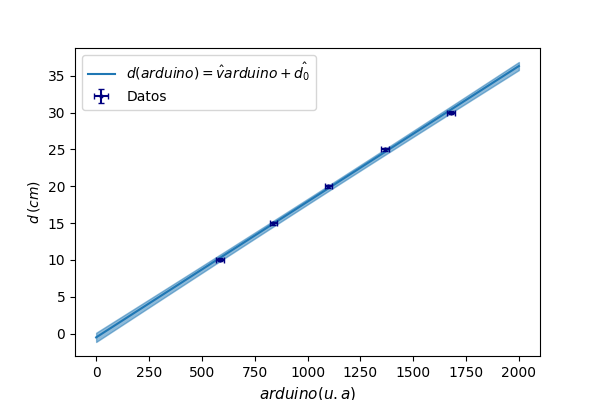
\includegraphics[width=0.9\linewidth]{Calibracion.png}
    \caption{Calibración del sistema}
    \label{fig:calibracion}
\end{figure}

Pendiente: $0.0184 \pm 0.0005$ \\

Ordenada al origen: ($-0.5 \pm 0.5$) cm\\

Distancia para 600: ($10.5 \pm 0.4$) cm \\

\newpage

\section{Resultados}

\subsection{Posicion}

\subsubsection*{Madera y Trineo}

En un primer caso dejamos el trineo deslizar sobre la mesa de madera. \\

\begin{figure}[H]
    \centering
    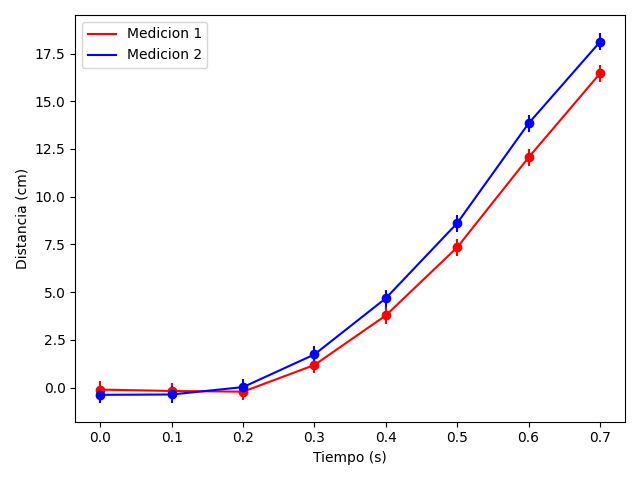
\includegraphics[width=0.4\linewidth]{TiempoVsDistanciaPisoMadera2PB_O.png}
    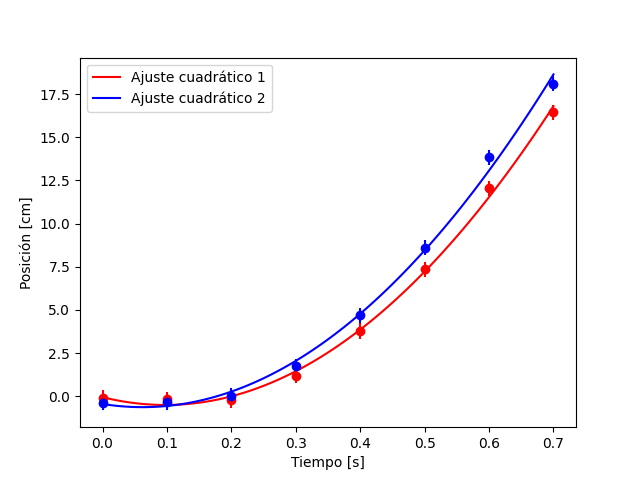
\includegraphics[width=0.44\linewidth]{ajuste2_PisoMadera2PB_O.png}
    \caption{$M = 161 \pm 1 g, m = 72 \pm 1 g$}
    \label{fig:2PB_O piso trineo}

\end{figure}

\begin{figure}[H]
    \centering
    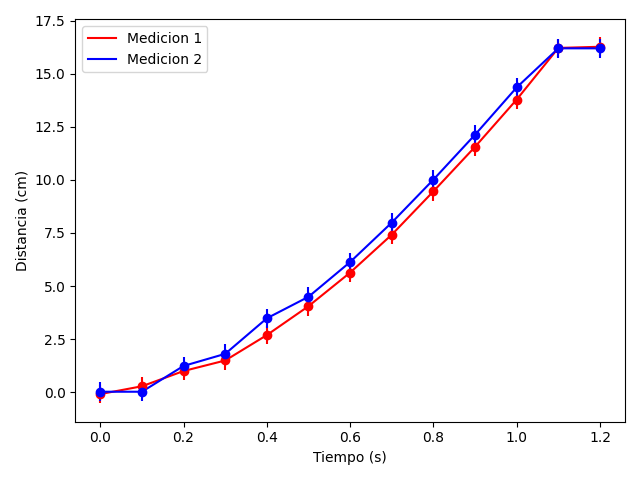
\includegraphics[width=0.4\linewidth]{TiempoVsDistanciaPisoMaderaMPB_O.png}
    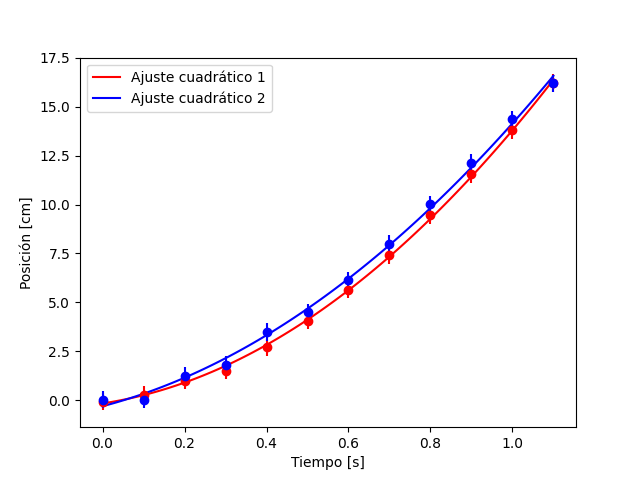
\includegraphics[width=0.44\linewidth]{ajuste2_PisoMaderaMPB_O.png}
    \caption{$M = 243 \pm 1 g, m = 95 \pm 1 g$}
    \label{fig:M_OP piso trineo}
\end{figure}

\begin{figure}[H]
    \centering
    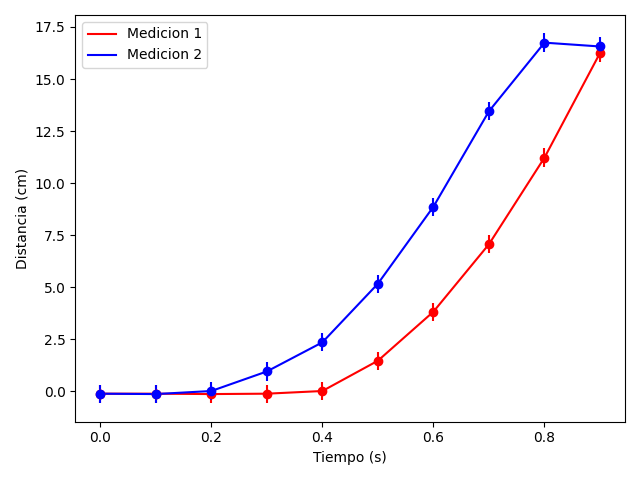
\includegraphics[width=0.4\linewidth]{TiempoVsDistanciaPisoMaderaV_2P.png}
    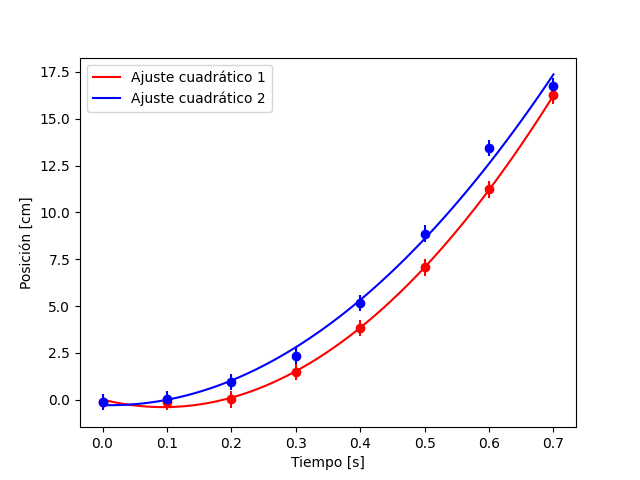
\includegraphics[width=0.44\linewidth]{ajuste2_PisoMaderaV_2P.png}
    \caption{$M = 109 \pm 1 g, m = 46 \pm 1 g$}
    \label{fig:V_2P piso trineo}
\end{figure}


De \ref{fig:2PB_O piso trineo}, \ref{fig:M_OP piso trineo} y \ref{fig:V_2P piso trineo} obtenemos valores de la aceleración del sistema. En promedio, la aceleración fue de $0.32 \pm 0.02$ cm/s\(^2\).

\subsubsection*{Papel y trineo}

Luego, le pegamos papel a la mesa y repetimos el experimento.

\begin{figure}[H]
    \centering
    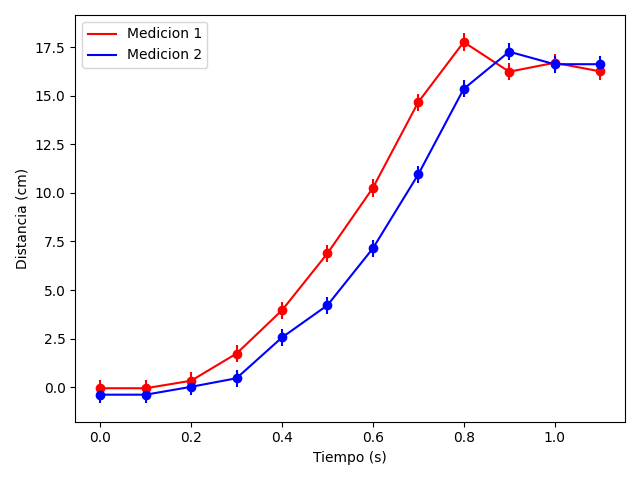
\includegraphics[width=0.4\linewidth]{TiempoVsDistanciaPisoHoja2PB_O.png}
    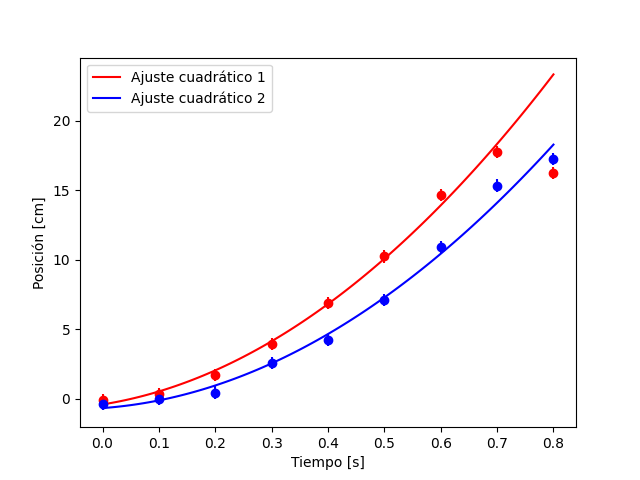
\includegraphics[width=0.44\linewidth]{ajuste2_PisoHoja2PB_O.png}
    \caption{$M = 161 \pm 1 g, m = 72 \pm 1 g$}
    \label{fig:2PB_O piso hoja}
\end{figure}

\begin{figure}[H]
    \centering
    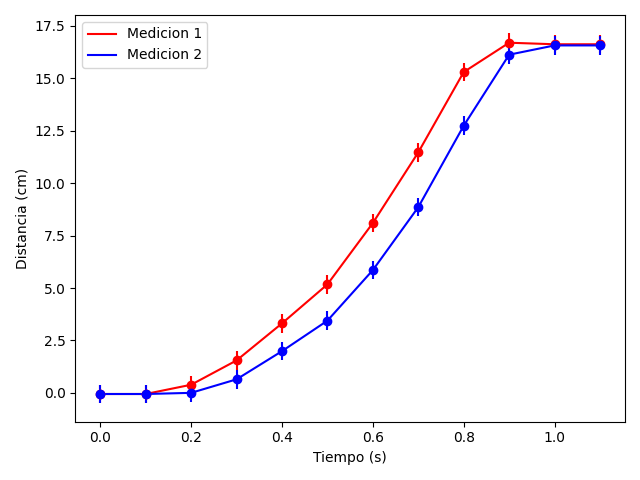
\includegraphics[width=0.4\linewidth]{TiempoVsDistanciaPisoHojaM_OP.png}
    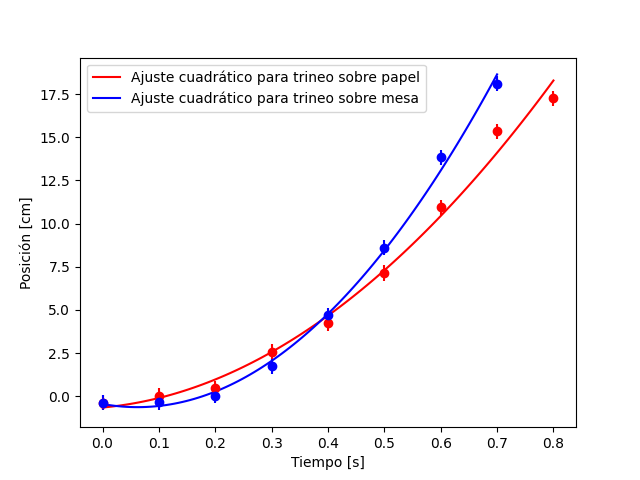
\includegraphics[width=0.44\linewidth]{ajuste2_PisoHojaM_OP.png}
    \caption{$M = 243 \pm 1 g, m = 95 \pm 1 g$}
    \label{fig:M_OP piso hoja}
\end{figure}

\begin{figure}[H]
    \centering
    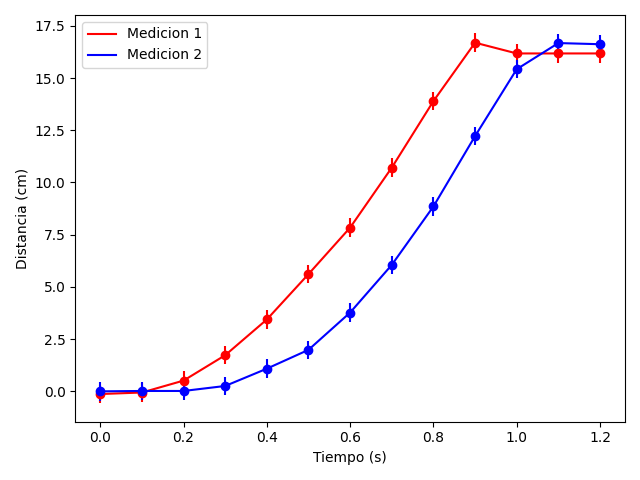
\includegraphics[width=0.4\linewidth]{TiempoVsDistanciaPisoHojaV_2P.png}
    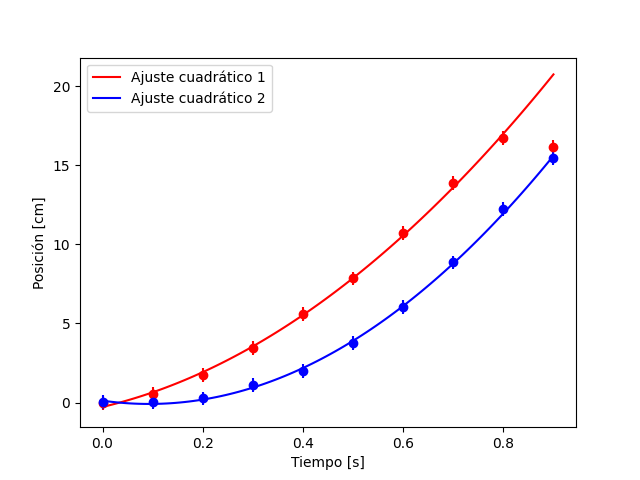
\includegraphics[width=0.44\linewidth]{ajuste2_PisoHojaV_2P.png}
    \caption{$M = 109 \pm 1 g, m = 46 \pm 1 g$}
    \label{fig:V_2P piso hoja}
\end{figure}


De \ref{fig:2PB_O piso hoja}, \ref{fig:M_OP piso hoja} y \ref{fig:V_2P piso hoja} obtenemos valores de la aceleración del sistema. En promedio, la aceleración fue de $0.22 \pm 0.03$ cm/s\(^2\).

\subsubsection*{Papel y Papel}

Por ultimo, pegamos otro papel al trineo y repetimos el experimento.

\begin{figure}[H]
    \centering
    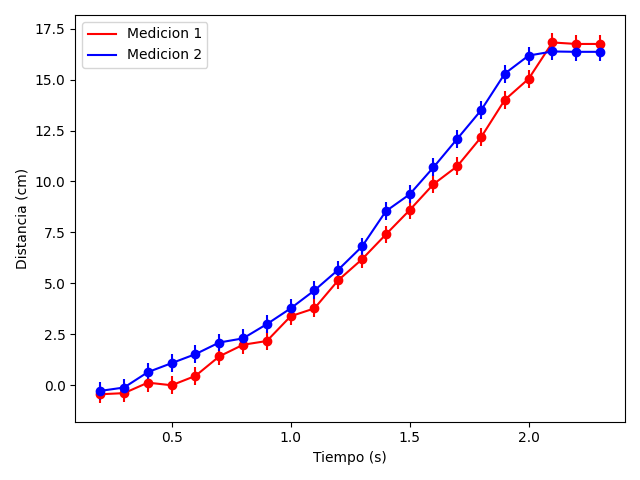
\includegraphics[width=0.4\linewidth]{TiempoVsDistanciaPapelPapelM_O.png}
    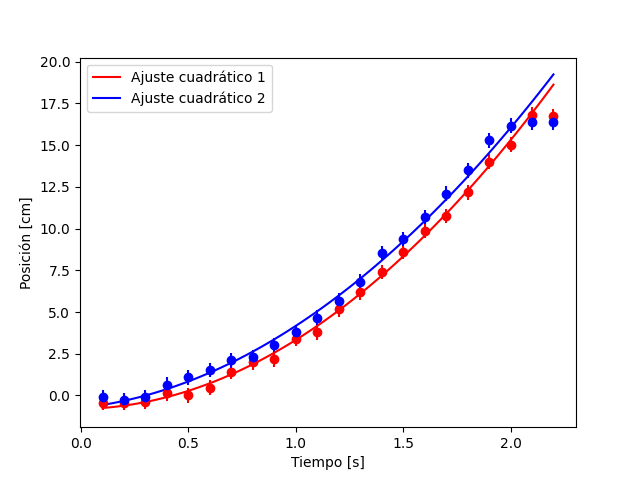
\includegraphics[width=0.44\linewidth]{ajuste2_PapelPapelM_O.png}
    \caption{$M = 243 \pm 1 g, m = 72 \pm 1 g$}
    \label{fig:M_O papel papel}
\end{figure}

\begin{figure}[H]
    \centering
    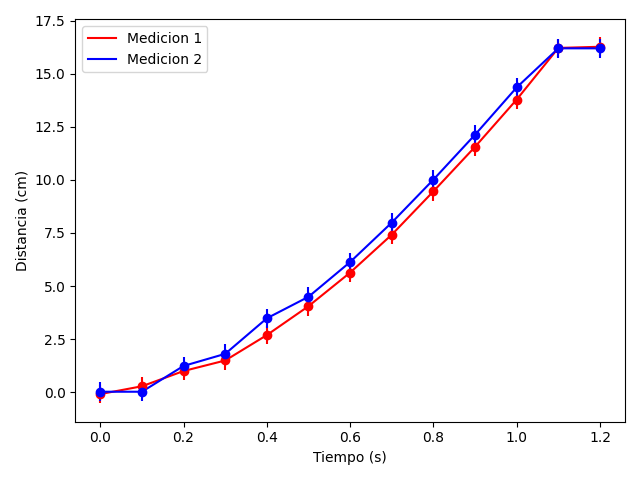
\includegraphics[width=0.4\linewidth]{TiempoVsDistanciaPapelPapelM_OP.png}
    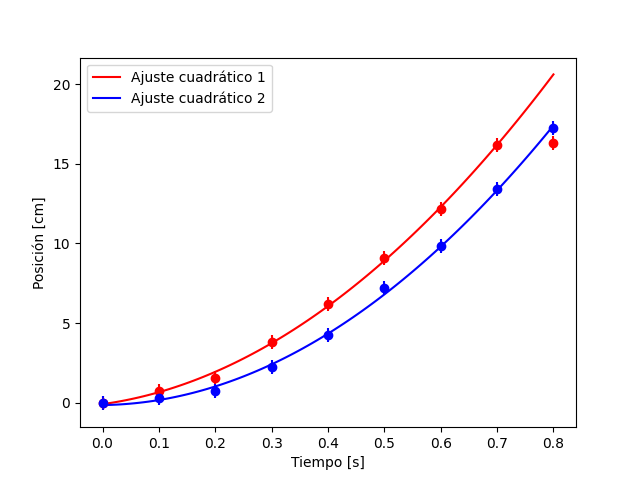
\includegraphics[width=0.44\linewidth]{ajuste2_PapelPapelM_OP.png}
    \caption{$M = 243 \pm 1 g, m = 95 \pm 1 g$}
    \label{fig:M_OP papel papel}
\end{figure}

\begin{figure}[H] %check esto
    \centering
    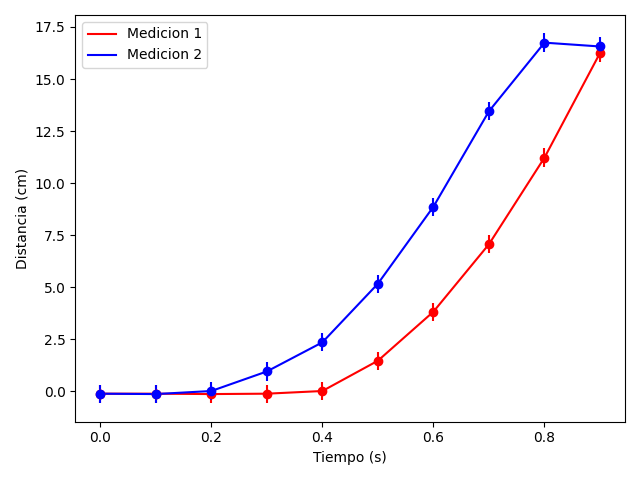
\includegraphics[width=0.4\linewidth]{TiempoVsDistanciaPapelPapelV_O.png}
    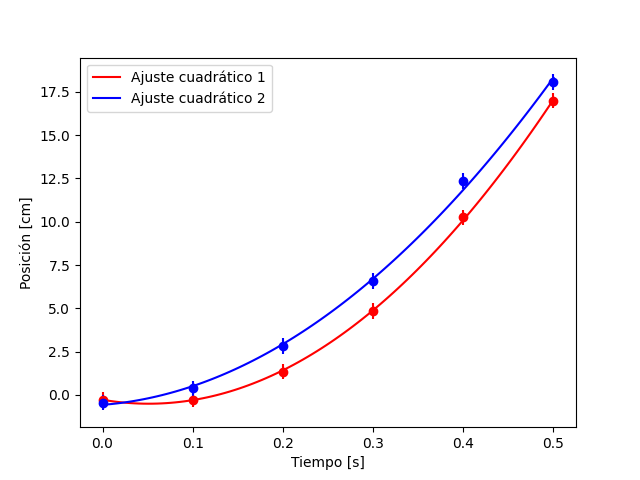
\includegraphics[width=0.44\linewidth]{ajuste2_PapelPapelV_O.png}
    \caption{$M = 109 \pm 1 g, m = 72 \pm 1 g$}
    \label{fig:TvDV_O papel papel}
\end{figure}


De \ref{fig:M_O papel papel}, \ref{fig:M_OP papel papel} y \ref{fig:TvDV_O papel papel} obtenemos valores de la aceleración del sistema. En promedio, la aceleración fue de $0.39 \pm 0.04$ cm/s\(^2\).

\subsection{Obtencion del $\mu_d$}

Sacando un promedio de los valores obtenidos de \ref{eq:mu_d} usando cada aceleración obtenemos un valor de $\mu_d$ para cada superficie.

\begin{figure}[H]
    \begin{minipage}{0.5\textwidth}
        \centering
        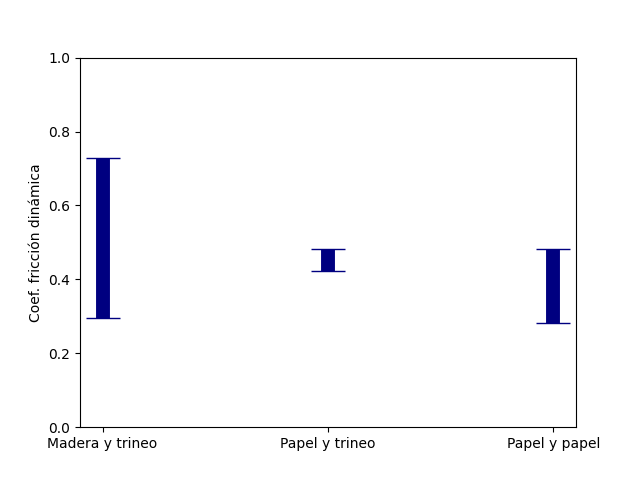
\includegraphics[width=0.9\linewidth]{ud_Combined.png}
        \caption{Promedio de $\mu_d$ para cada superficie}
        \label{fig:mu_d promedio}
    \end{minipage}\hfill
    \begin{minipage}{0.5\textwidth}
        \centering
        \begin{table}[H]
            \centering
            \begin{tabular}{|c|c|}
                \hline
                \textbf{Superficie} & \textbf{$\mu_d$}\\
                \hline
                Madera y trineo & $0.4 \pm 0.1$\\
                Papel y trineo & $0.45 \pm 0.03$ \\
                Papel y Papel & $0.5 \pm 0.2$ \\
                \hline
            \end{tabular}
            \caption{Valores de $\mu_d$ y sus incertezas para cada superficie}
            \label{tab:mu_d}
        \end{table}
    \end{minipage}
\end{figure}

\section{Conclusiones}

A través de las mediciones de aceleración en diversas configuraciones de masa y superficie, se obtuvieron valores para el $\mu_d$, destacándose variaciones entre las diferentes superficies analizadas.

Los resultados obtenidos evidencian que la fricción varía dependiendo de la textura de las superficies en contacto. Por ejemplo, el valor de $\mu_d$ en la superficie de madera fue de 0.4 ± 0.1, mientras que en papel sobre papel fue mayor, alcanzando un promedio de 0.5 ± 0.2. Esta variación en el coeficiente es indicativa de la influencia de la rugosidad y la naturaleza del material en la interacción de fricción.

Por las incertezas de los resultados, podemos comprender la importancia de las condiciones experimentales y cómo pequeñas variaciones pueden impactar en los resultados, reforzando el valor de una correcta medición y calibración en estudios físicos.


\end{document}